
\section{Aleatoriedad y procesos estocásticos}

\subsection{Desigualdad de Jensen}
Sea la función convexa $f(S)$ (que se curva hacia arriba, con forma de cuenco) de la variable aleatoria $S$, entonces
\[\mathbb{E}[f(S)] \geq f(\mathbb{E}[S])\]
De hecho, la diferencia es de
\[\frac{1}{2}f''(\mathbb{E}[S])\mathbb{E}[\epsilon]\]
donde $\epsilon$ es la desviación de $S$ de la media, i.e $S=\mathbb{E}[S]+\epsilon$.


\subsection{Propiedad de Markov}
\textit{El futuro depende solo del presente, no del pasado.} Se usa en los caminos aleatorios para decir que el valor $S_t+1$ solo depende de $S_t$, es decir,
\[\mathbb{P}(X_{t+s} \in A \mid X_t = x, X_{t_1} = x_1, \ldots, X_{t_n} = x_n) 
= \mathbb{P}(X_{t+s} \in A \mid X_t = x)\]



\subsection{Propiedad de martingala}
\textit{Lo que esperas tener en el futuro, sabiendo todo hasta ahora, es exactamente lo que tienes ahora}. Es decir, el valor esperado de algo en un juego justo es exactamente lo que tienes ahora:
\[\mathbb{E}[S_i|S_j, j<i]=S_j\]



\subsection{Lema de Itô}\label{Ito}
Sea
\[dS = a(S,t)dt + b(S,t)d\mathnormal{X}\]
entonces
\[dV = \left( \frac{dV}{dt} +  a\frac{dV}{dS} + \frac{1}{2}b^2\frac{d^2V}{dS^2} \right)dt + b\frac{dV}{dS}d\mathnormal{X}\]
En el documento~\ref{CalcIto} se encuentra la fórmula para dimensiones mayores.

\subsection{Algunos ejemplos de caminos aleatorios}

\begin{itemize}
    \item \textbf{Brownian Motion with Drift}: $dS = \mu dt + \sigma d\mathnormal{X}$
    \begin{figure}[H]
        \centering
        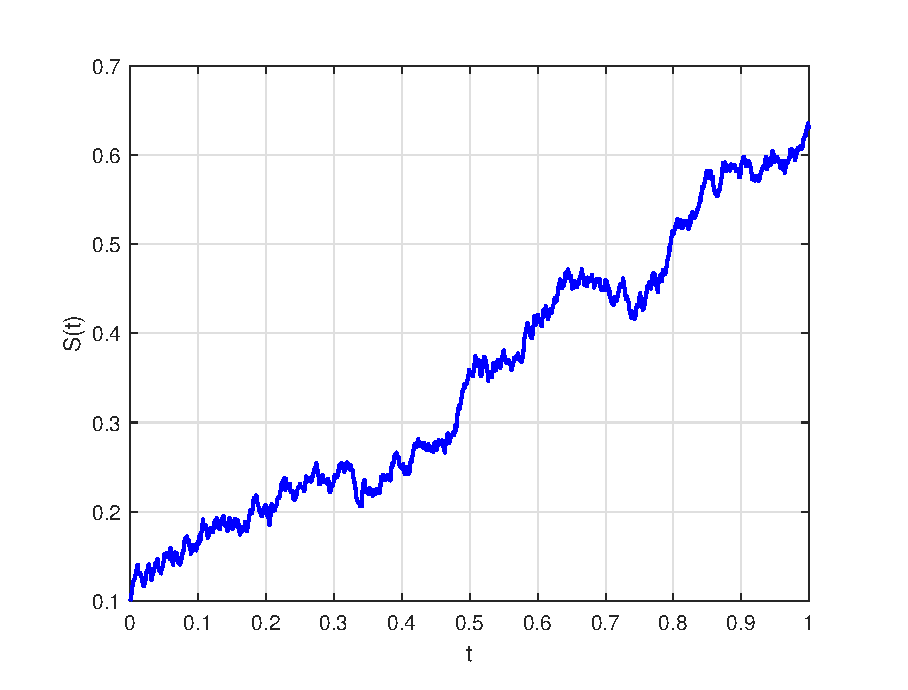
\includegraphics[width=0.5\linewidth]{Imagenes/3_Aleatoriedad/BrownianMotionDrift.eps}
        \caption{Brownian Motion with Drift}
    \end{figure}
    \item \textbf{The Lognormal Random Walk}: $dS = S\mu dt + S\sigma d\mathnormal{X}$
    \begin{figure}[H]
        \centering
        \includegraphics[width=0.5\linewidth]{Imagenes/3_Aleatoriedad/LognormalRandomWalk.eps}
        \caption{The Lognormal Random Walk}
    \end{figure}
    \item \textbf{A Mean-reverting Random Walk}: reversion a la media, cuando se esta fuera del crecimiento normal el camino tiende a corregirse.\\
    Su EDE es $dS = \kappa(\theta+S) dt + \sigma d\mathnormal{X}$, donde $\kappa$ es la velocidad de reversión a la media, $\theta$ es la tasa de interés a largo plazo y $\sigma$ es la volatilidad. Un ejemplo común es el modelo Vasicek para el ratio de interés, $dr = \kappa(\theta+r) dt + \sigma d\mathnormal{X}$
    \begin{figure}[H]
        \centering
        \includegraphics[width=0.5\linewidth]{Imagenes/3_Aleatoriedad/MeanRevertingWalk.eps}
        \caption{Mean-reverting Random Walk}
    \end{figure}
\end{itemize}










